\documentclass[letterpaper, 10pt, draftclsnofoot, compsoc, onecolumn]{IEEEtran}
\usepackage[latin1]{inputenc}
\usepackage[T1]{fontenc}
\usepackage[english]{babel}
\usepackage{amsmath}
\usepackage{amssymb,amsfonts,textcomp}
\usepackage{color}
\usepackage{array}
\usepackage{comment}
\usepackage{supertabular}
\usepackage{hhline}
\usepackage{hyperref}
\usepackage{url}
\usepackage{fancyhdr}
\def\name{Steven Powers, Josh Matteson, Evan Tschuy}
\hypersetup{
  colorlinks=true, linkcolor=blue, citecolor=blue, filecolor=blue, urlcolor=blue, pdfauthor = {\name},
  pdfkeywords = {cs461 ``senior capstone'' requirements},
  pdftitle = {CS 461 Requirements Document},
  pdfsubject = {CS 461 Requirements Document},
  pdfpagemode = UseNone}
\usepackage[pdftex]{graphicx}

% Outline numbering
\setcounter{secnumdepth}{5}
\renewcommand\thesection{\arabic{section}}
\renewcommand\thesubsection{\arabic{section}.\arabic{subsection}}
\renewcommand\thesubsubsection{\arabic{section}.\arabic{subsection}.\arabic{subsubsection}}
\renewcommand\theparagraph{\arabic{section}.\arabic{subsection}.\arabic{subsubsection}.\arabic{paragraph}}

\makeatletter
\newcommand\arraybslash{\let\\\@arraycr}
\makeatother
% Page layout (geometry)
\setlength\voffset{-1in}
\setlength\hoffset{-1in}
\setlength\topmargin{0.5in}
\setlength\oddsidemargin{1in}
\setlength\evensidemargin{1in}
\setlength\textheight{8.278in}
\setlength\textwidth{6.5in}
\setlength\footskip{0.561in}
\setlength\headheight{0.5in}
\setlength\headsep{0.461in}
% Footnote rule
\setlength{\skip\footins}{0.0469in}
\renewcommand\footnoterule{\vspace*{-0.0071in}\setlength\leftskip{0pt}\setlength\rightskip{0pt plus 1fil}\noindent\textcolor{black}{\rule{0.25\columnwidth}{0.0071in}}\vspace*{0.0398in}}

% Pages styles

\makeatletter
%\newcommand\ps@Standard{
%  \renewcommand\@oddhead{\rmfamily\color{black}Many Voices Publishing Platform\hfill \hfill }
%  \renewcommand\@evenhead{\@oddhead}
%  \renewcommand\@oddfoot{}%{\textcolor{black}{SSRS Page }}{\textcolor{black}{\thepage{}}}}
%  \renewcommand\@evenfoot{\@oddfoot}
%  \renewcommand\thepage{\arabic{page}}
%}

\pagestyle{empty}
\renewcommand{\headrulewidth}{0pt}
\lhead{Many Voices Publishing Platform}

\lfoot{SSRS}
\cfoot{Page}
\rfoot{\thepage}

%\newcommand\ps@Convertviii{
%  \renewcommand\@oddhead{}
%  \renewcommand\@evenhead{\@oddhead}
%  \renewcommand\@oddfoot{}
%  \renewcommand\@evenfoot{\@oddfoot}
%  \renewcommand\thepage{\arabic{page}}
%}

\newcommand\ps@FirstPage{
  \renewcommand\@oddhead{}
  \renewcommand\@evenhead{\@oddhead}
  \renewcommand\@oddfoot{}
  \renewcommand\@evenfoot{\@oddfoot}
  \renewcommand\thepage{\arabic{page}}
}
\makeatother
%\pagestyle{Standard}
\setlength\tabcolsep{1mm}
\renewcommand\arraystretch{1.3}
% footnotes configuration
\makeatletter
\renewcommand\thefootnote{\arabic{footnote}}
\makeatother
\title{MANY VOICES PUBLISHING PLATFORM}
\author{Steven Powers}
\date{2016-10-27}


\begin{document}
\clearpage\setcounter{page}{1}%\pagestyle{Standard}
\thispagestyle{FirstPage}


\bigskip
\bigskip
\clearpage
{\centering\bfseries\color{black}\huge
MANY VOICES PUBLISHING PLATFORM
\par}
\bigskip
\bigskip
{\centering\bfseries\color{black}\Large
SYSTEMS AND SOFTWARE \ REQUIREMENTS SPECIFICATION (SSRS)
\par}
\bigskip
\bigskip
\bigskip
\bigskip
\bigskip
{\centering\bfseries\color{black}Version 0.5\par}
{\centering\bfseries\color{black}October 27, 2016\par}
\bigskip
\bigskip
{\centering\bfseries\color{black}Prepared for:\par}
{\centering\bfseries\color{black}Dr. Carlos Jensen, D. Kevin McGrath, and Dr. Kirsten Winters\par}
{\centering\bfseries\color{black}CS461 Senior Capstone\par}
\bigskip
\bigskip
{\centering\bfseries\color{black}Prepared by:\par}
{\centering\bfseries\color{black}Commix\par}
{\centering\bfseries\color{black}Josh Matteson, Steven Powers, and Evan Tschuy\par}
{\centering\bfseries\color{black}Oregon State University\par}
{\centering\bfseries\color{black}Corvallis, OR \ 97330\par}
\bigskip

\begin{abstract}
\noindent An overview of the requirements for the Many Voices Publishing Platform. 
Introduces the Many Voices Publishing Platform, describes in detail the purpose, 
product functions, user characteristics, assumptions and dependencies, 
and system level (non-functional) requirements and lists specific requirements 
that are outside of the platform, system features, and an overview of the development life cycle.
\end{abstract}



\begin{comment}
\clearpage{\centering\bfseries\color{black}Many Voices Publishing Platform SSRS\par}
\bigskip
{\centering\bfseries\color{black}RECORD OF CHANGES\par}
\bigskip
\begin{flushleft}
\tablehead{}
\begin{supertabular}{|m{0.47685984in}|m{0.6087598in}|m{1.3587599in}|m{0.23375985in}|m{2.0462599in}|m{0.7337598in}|m{0.6330598in}|}
\hline
~

\centering \color{black} Change number &
~

\centering \color{black} Date completed &
~

\centering \color{black} Location of change
(e.g., page or figure \#) &
\centering \bfseries\color{black} A\newline
M\newline
D &
~

~

\centering \color{black} Brief description of
change &
~

\centering \color{black} Approved by (initials)
&
~

\centering\arraybslash \color{black} Date
Approved\\\hline
~
 &
~
 &
~
 &
~
 &
~
 &
~
 &
~
\\\hline

\end{supertabular}
\end{flushleft}
{\color{black}
{*}{\textbf{A}}{
- ADDED
\ }{\textbf{M}}{ -
MODIFIED
\ }{\textbf{D}}{ -
DELETED}}
\end{comment}

\clearpage
{\centering
{\MakeUppercase{\ }}{\MakeUppercase{Many Voices Publishing Platform SSRS}}
\par}

{\centering
TABLE OF CONTENTS
\par}

\setcounter{tocdepth}{9}
%\renewcommand\contentsname{}
\tableofcontents

%\medskip

\clearpage

\setcounter{page}{1}\pagestyle{fancy}
\section[Introduction]{\rmfamily\bfseries\color{black} Introduction}

\subsection[IDENTIFICATION]{\rmfamily\bfseries\color{black} IDENTIFICATION}


{\noindent
The software system being considered for development is referred to as the Many Voices
Publishing Platform. \ The customer providing specifications
for the system is Dr. Carlos Jensen that is reachable at his email jensenca@engr.orst.edu \
The ultimate customer, or end-user, of the system will be any user that wants an easier
way to combine materials into a book. \ This is a new project effort, so the
version under development is version 0.5 release 0. As the system may be based off of Ward Cunningham's 
Federated Wiki, the project will have a substantial head start, signified by the 0.5 version number \cite{Federated}.}

\subsection[PURPOSE]{\rmfamily\bfseries\color{black} PURPOSE}

{\noindent 
The purpose of the system under
development is to provide a collaborative authoring platform that allows for users to
combine various materials into a book. \ While the system will be used by professors and
instructors in majority, this document is intended to be read and understood by software
designers and coders. \ The document will also be vetted or
approved by Dr. Carlos Jensen, D. Kevin McGrath, and Dr. Kirsten Winters.}

\subsection[SCOPE]{\rmfamily\bfseries\color{black} SCOPE}

{\noindent 
The project is sponsored by Dr. Carlos Jensen, being developed by Josh Matteson,
Steven Powers, and Evan Tschuy for completion of CS461 Senior capstone project class.
The product is to be operated via a website for wide availability and use.}

\subsection[DEFINITIONS, ACRONYMS, AND ABBREVIATIONS]{\rmfamily\bfseries\color{black} DEFINITIONS, ACRONYMS, AND ABBREVIATIONS}

\bigskip

\begin{center}

\tablehead{}
\begin{supertabular}{|p{3cm}|p{12cm}|}
\hline
Term or Acronym & Definition\\\hline
Alpha Test & Limited release(s) to selected, outside testers (Friends and Family)\\ \hline
Beta Test & Limited release(s) to cooperating customers wanting early access to developing systems (Professors 
and other educators)\\ \hline
Final Test & Release of full functionality to customer for approval \\ \hline
SDD & Software Design Document \\ \hline
SSRS & System and Software Requirements Specification \\ \hline
PDF & Portable Document Format, that is able to combine text, graphics, and other information into a single document \\ \hline
PCI & Payment Card Industry, is a proprietary information security standard for credit cards in an effort to reduce credit card fraud \\ \hline
Federated & Individual parts that stand as an individual but can be combined into a single unit \\ \hline
Wiki & A collaborative content editing platform \\ \hline
Scrap & A section of a textbook, which can contain formatted text (markdown or latex), and media \\ \hline
Section & An ordered collection of Scraps belonging to a chapter\\ \hline
Chapter & An ordered collection of Sections and Scraps\\ \hline
Media & A standalone image, figure, or video. Can be embedded in a Scrap\\ \hline
Web Application & An interactive program that can be accessed and is based through a web server instead of 
being stored on a user's desktop\\ \hline
Source Control & An element of software design management, version control, and is the 
management of changes to documents, large web sites, computer programs, and other 
collections of data \\ \hline
User Interface (UI)  & The means by which the user and a computer system interact, in particular the use of 
input devices and software\\ \hline
\end{supertabular}

\end{center}
\subsection[REFERENCES]{\rmfamily\bfseries\color{black} REFERENCES}

{\noindent
[1] C.  Jeffery, Systems and Software Requirements Specification (SSRS) Template, 2nd ed. Moscow: University of Idaho, 2016, pp. 1-22.}

\subsection[OVERVIEW AND RESTRICTIONS]{\rmfamily\bfseries\color{black} OVERVIEW AND RESTRICTIONS}


{\noindent
This document is for limited release only to Oregon State University professors and
associated staff of D. Kevin McGrath, Dr. Kirsten Winters, and Jon Dodge, personnel
working on the project, and the client, Dr. Carlos Jensen.}


\bigskip

%\noindent {\color{black}
%Section 2 of this document describes the system under development from a
%holistic point of view. \ Functions, characteristics, constraints,
%assumptions, dependencies, and overall requirements are defined from
%the system-level perspective.}


\bigskip

%\noindent {\color{black}
%Section 3 of this document describes the specific requirements of the
%system being developed. \ Interfaces, features, and specific
%requirements are enumerated and described to a degree sufficient for a
%knowledgeable designer or coder to begin crafting an architectural
%solution to the proposed system.}


\bigskip


%\noindent {\color{black}
%Section 4 provides the requirements traceability information for the
%project. \ Each feature of the system is indexed by the SSRS
%requirement number and linked to its SDD and test references.}


\bigskip

%\noindent {\color{black}
%Sections 5 and up are appendices including original information and
%communications used to create this document.}

\clearpage
\section[OVERALL DESCRIPTION]{\rmfamily\bfseries\color{black} OVERALL DESCRIPTION}

\subsection[PRODUCT PERSPECTIVE]{\rmfamily\bfseries\color{black} PRODUCT PERSPECTIVE}

{\noindent
The main differentiator from traditional textbook publication methods are the products'
micro-writing abilities. A traditional textbook is written by one expert, using a defined
curriculum that fits the needs of the author. The curriculum is a generic version of a
multitude of classes that is somewhat useful for many professors, rather than very useful
for few professors. Instead, our solution will give the tools necessary for individual 
professors to create the textbook they need to match the curriculum desired. This allows 
for textbooks that more closely track the intricacies of how classes are taught by 
different individuals.}

\subsection[PRODUCT FUNCTIONS]{\rmfamily\bfseries\color{black} PRODUCT FUNCTIONS}

{\noindent 
The product will be a document construction service. The most basic usage will be the 
creation of a textbook out of pre-existing chapters, by searching and selecting from a 
list. Alternatively, chapters can created using pre-existing sections and media.
A chapter or section can be created using a simple input interface that
accepts text and LaTeX markup, along with the upload of media like image or
perhaps video content.}

\subsection[USER CHARACTERISTICS]{\rmfamily\bfseries\color{black} USER CHARACTERISTICS}

{\noindent 
The expected user of the service will be a professor. Professors, in general, have
decent means technical skills. Thus, the interface of the product
will be highly graphically driven, using modern interface paradigms as defined
by industry leaders, such as Google's Material Design \cite{GoogleMaterial}. 
The interface will allow users to not think about the technical specificities of the product, 
but more-so on the content they are using, the authors of the content, and how they are using it.}

\subsection[CONSTRAINTS]{\rmfamily\bfseries\color{black} CONSTRAINTS}

{\noindent 
A regular web browser will be the means of access for users. For the backend
server, the main requirement is availability - as a web application, it has no
safety- or life-critical components. A high (99.99\%) availability should be provided,
but otherwise availability, safety, and specific hardware are not main concerns.}

\bigskip

{\noindent 
The software can, as a web application, be written in a high-level language, with
minimal inter-application communication. In the case that the software is built
on top of other applications, such as Git, inter-process communication should be
handled in a generic way that provides a high-security barrier, preventing malicious
users from accessing other, non-specified applications.}

\subsection[ASSUMPTIONS AND DEPENDENCIES]{\rmfamily\bfseries\color{black} ASSUMPTIONS AND DEPENDENCIES}

{\noindent
The product will be designed to run on a generic Linux-with-web server environment.
Ward Cunningham's Federated Wiki, a similar project being drawn upon for inspiration, can run
on any system with Ruby and CouchDB (a popular NoSQL database) \cite{Federated}. 
With the product being either partially or wholly based on the Federated Wiki, similar system
requirements are anticipated \cite{Federated}.

\subsection[SYSTEM LEVEL (NON{}-FUNCTIONAL) REQUIREMENTS]{\rmfamily\bfseries\color{black} SYSTEM LEVEL (NON-FUNCTIONAL) REQUIREMENTS}


\subsubsection[Site Dependencies]{\rmfamily\bfseries\color{black} Site Dependencies}
As a web application, the product has no hard requirements other than high-speed
network access and an instance of the CouchDB database management system.
\begin{itemize}
  \item Hardware: standard virtual machine(s) running on cloud provider (ex: Amazon EC2 
  t2.medium)
  \item Possible Database: CouchDB 2.0
\end{itemize}

\subsubsection[Safety, Security and Privacy Requirements]{\rmfamily\bfseries\color{black} Safety, Security and Privacy Requirements}

{\noindent 
Private information shall be held to any relevant security standards. For instance,
any credit card information processed by the product in the textbook creation process
will be held to PCI compliance standards. Passwords shall be stored in a securely hashed,
non-reversible method, such that infiltration of the product by an unauthorized
third party will not be able to result in the theft of user passwords or other private
information.}

\subsubsection[Performance Requirements]{\rmfamily\bfseries\color{black} Performance Requirements}

{\noindent
A standard user load shall be defined as up to 100 simultaneous users. User information
will include things such as text documents, media uploads, and user account data.

Under a standard load:
\begin{itemize}
  \item 95\% of save operations (excepting media upload time) shall be responsive in 
  nature.
  \item 95\% of initial page loads shall shall be responsive in 
  nature.
  \item 95\% of user account operations (login, creation, deletion, etc) shall be 
  responsive in nature.
\end{itemize}}

\subsubsection[System and Software Quality]{\rmfamily\bfseries\color{black} System and Software Quality}

The software shall maintain 99.99\% accessibility from the major modern web browsers, including Mozilla FireFox, 
Google Chrome, and Microsoft Edge.
As a non-safety-critical product, reliability shall be attempted but not promised
to end users. Testing shall be handled through a suite of automated unit and integration testing, as well as
through manual checking of newly written and critical features.

\subsubsection[Packaging and Delivery Requirements]{\rmfamily\bfseries\color{black} Packaging and Delivery Requirements}

{\noindent 
The executable system and all associated documentation (i.e., SSRS,
code listing, test plan (data and results), and user manual) will be
delivered to the customer on CD{\textquoteright}s and/or via email, as
specified by the customer at time of delivery. \ Although document
{\textquotedblleft}drops{\textquotedblright} will occur throughout the
system development process, the final, edited version of the above
documents will accompany the final, accepted version of the executable
system.}

\subsubsection[Personnel{}-related requirements]{\rmfamily\bfseries\color{black} Personnel-related requirements} 

{\noindent
The system under development has no special personnel-related characteristics. }

\subsubsection[Training{}-related
requirements]{\rmfamily\bfseries\color{black}
Training-related requirements}
%\noindent {\color{black}
%{\textit{This paragraph shall specify the
%system requirements, if any, pertaining to training. \ Examples include
%training software, tutorials, or help information to be included in the
%system.}}{ \ \ }}

\noindent {\color{black}
No training materials or expectations will be tied to this project other
than the limited help screens built into the software and the
accompanying user manual.}

\subsubsection[Logistics{}-Related Requirements]{\rmfamily\bfseries\color{black} Logistics-Related Requirements}

\noindent {\color{black}
The software shall run on a standard Amazon Web Services backend instance with
another standard instance serving as the database.


\subsubsection[Other Requirements]{\rmfamily\bfseries\color{black} Other Requirements}

{\noindent No other system requirements are anticipated.}

\subsubsection[Precedence and Criticality of Requirements]{\rmfamily\bfseries\color{black} Precedence and Criticality of Requirements}

{\noindent The main critical requirements of the system are those relating to payment processing secrecy.}

\clearpage


%Section 3
\section[SPECIFIC REQUIREMENTS]{\rmfamily\bfseries\color{black} SPECIFIC REQUIREMENTS}


\subsection[EXTERNAL INTERFACE REQUIREMENTS]{\rmfamily\bfseries\color{black} EXTERNAL INTERFACE REQUIREMENTS}

\subsubsection[Hardware Interfaces]{\rmfamily\bfseries\color{black} Hardware Interfaces}
{\noindent 
User should have a basic computer 
with no extensive requirements. The project should be able to run on a standard virtual machine 
instance.}

\subsubsection[Software Interfaces]{\rmfamily\bfseries\color{black} Software Interfaces}
{\noindent 
Web front-end using JavaScript or JavaScript variant.}

\subsubsection[User Interfaces]{\rmfamily\bfseries\color{black} User Interfaces}
{\noindent 
Angular2 - Single Page Application, or other similar variant}

\subsubsection[Other Communication Interfaces]{\rmfamily\bfseries\color{black} Other Communication Interfaces}
{\noindent 
Git, email, comments}


\bigskip

\clearpage
%\setcounter{page}{1}\pagestyle{Convertv}
\subsection[SYSTEM FEATURES]{\rmfamily\bfseries\color{black} SYSTEM FEATURES}


\begin{comment}
\subsubsection[\ Use Case Diagrams]{{\ }{Use Case Diagrams}}
{\noindent 
[insert 1+ use case diagrams here]}
\end{comment}

\subsubsection[System feature 1: General Website Features]{\rmfamily\bfseries\color{black} General Website Features}

\begin{itemize}
\item These may come free if we duplicate and edit the Federated Wiki.
\item Material/otherwise nice looking design template
\item User account management
\item Create new account
\item Edit existing account
\item Login / logout functionality
\end{itemize}

\subsubsection[System feature 2: Compile a book]{\rmfamily\bfseries\color{black} Compile a Book}
\begin{itemize}
\item Search functionality for finding existing textbooks
\item Ability to duplicate and edit existing textbooks
\item Add a new blank textbook
\end{itemize}

\subsubsection[System feature 3: Textbook Compilation Interface]{\rmfamily\bfseries\color{black} Textbook Compilation Interface}
\begin{itemize}
\item Edit/New Chapter:
\item Table of Contents view, with access to New Chapter and Edit Chapter
\item Button to Add New Section/Scrap
\item Button to Search Sections/Scraps
\item User-friendly interface to add Section/Scrap to desired location in Chapter
\end{itemize}

\subsubsection[System feature 4: Search Feature]{\rmfamily\bfseries\color{black} Search}
\begin{itemize}
\item By keyword, author, tag, field; ranked by relevance and/or community voting
\item Scrap/Section search
\item Textbook search
\end{itemize}

\subsubsection[System feature 5: Publishing Interface]{\rmfamily\bfseries\color{black} Publishing Interface}
\begin{itemize}
%Need to talk to Carlos about this
%\item Indicate number of copies/digital access for students, determine price
\item Save textbook as PDF/send to printer
\item Optional future feature: payment processor integration
\end{itemize}

\subsubsection[System feature 6: Scrap Editor]{\rmfamily\bfseries\color{black} Scrap Editor}
\begin{itemize}
\item "Pretty" view for adding formatted text, media, etc to a scrap
\item "Raw" view for managing scrap ordering
\item Tag management (add, delete, search? tags)
%\item Price management
\end{itemize}

\bigskip


%Use Cases To Add
\begin{comment}
\bigskip
\noindent {\color{black}
{\textit{For each feature, you should either
provide a Use Case Description
}}{\textbf{\textit{or}}}{\textit{
a Non-task feature description, whichever is more appropriate.}}}



\bigskip

\begin{flushleft}
\tablehead{}
\begin{supertabular}{|m{3.17056in}|m{3.1740599in}|}
\hline
\bfseries\color{black} Use Case Description & 
\paragraph[Non{}-task feature
description]{\rmfamily\bfseries\color{black}
Non-task feature description}
\\\hline
{\bfseries\color{black} Name}

{\color{black} Actors}

{\color{black} Goals}

{\color{black} Preconditions}

{\bfseries\color{black} Summary}

{\color{black} Related use cases}

{\bfseries\color{black} Steps}

{\color{black} \ \ \ 1. ...}

{\color{black} \ \ \ 2. ...}

{\color{black} Alternatives}

{\color{black} Postconditions}

~
 &
\paragraph[\ Introduction/Purpose of this
feature]{{\ }{Introduction/Purpose
of this feature}}
{\color{black} [ insert your text here ]}

\paragraph[Input/Output sequence for this
feature]{\rmfamily\bfseries\color{black}
Input/Output sequence for this feature}
{\color{black} [ insert your text here ]}

\paragraph[Design constraints of this
feature]{\rmfamily\bfseries\color{black} Design
constraints of this feature}
{\color{black} [ insert your text here ]}

\paragraph[Performance requirements of this
feature]{\rmfamily\bfseries\color{black}
Performance requirements of this feature}
{\color{black} [ insert your text here ]}

\paragraph[Detailed functional requirements of this
feature]{\rmfamily\bfseries\color{black}
Detailed functional requirements of this feature}




\paragraph[]{\rmfamily\bfseries\color{black} }

\color{black} [ insert your text here ]\\\hline
\end{supertabular}
\end{flushleft}

\bigskip
\end{comment}


\begin{comment}

\subsubsection[System feature 2: [ insert feature name here
{]}]{\rmfamily\bfseries\color{black} System
feature 2: [ insert feature name here ]}
\paragraph[Introduction/Purpose of this feature]
{\rmfamily\bfseries\color{black}Introduction/Purpose of this feature}
\noindent {\color{black}
[ insert your text here ]}

\paragraph[Input/Output sequence for this feature]{\rmfamily\bfseries\color{black}Input/Output sequence for this feature}
\noindent {\color{black}
[ insert your text here ]}

\paragraph[Design constraints of this
feature]{\rmfamily\bfseries\color{black} Design
constraints of this feature}
\noindent {\color{black}
[ insert your text here ]}

\paragraph[Performance requirements of this
feature]{\rmfamily\bfseries\color{black}
Performance requirements of this feature}
\noindent {\color{black}
[ insert your text here ]}

\paragraph[Detailed functional requirements of this
feature]{\rmfamily\bfseries\color{black}
Detailed functional requirements of this feature}


{\rmfamily\bfseries\color{black} System
feature [m]: [ insert feature name here ]}

\paragraph[\ Introduction/Purpose of this feature]{\rmfamily\bfseries\color{black}Introduction/Purpose of this feature}
\noindent {\color{black}
[ insert your text here ]}

\paragraph[Input/Output sequence for this
feature]{\rmfamily\bfseries\color{black}
Input/Output sequence for this feature}

\paragraph[Design constraints of this
feature]{\rmfamily\bfseries\color{black} Design
constraints of this feature}
\noindent {\color{black}
[ insert your text here ]}

\paragraph[Performance requirements of this
feature]{\rmfamily\bfseries\color{black}
Performance requirements of this feature}
\noindent {\color{black}
[ insert your text here ]}

\paragraph[Detailed functional requirements of this
feature]{\rmfamily\bfseries\color{black}
Detailed functional requirements of this feature}
\noindent {\color{black}
[ insert your text here ]}

\end{comment}


\clearpage
%\setcounter{page}{1}\pagestyle{Convertvii}
\section[APPENDIX A. \ Gantt Chart]{\rmfamily\bfseries\color{black}
APPENDIX A. \ Gantt Chart}

\bigskip


\begin{figure}[ht!]
\centering
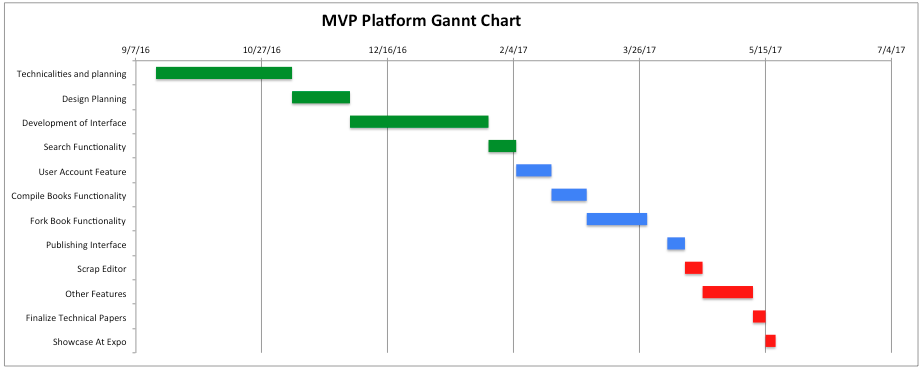
\includegraphics[width=160mm]{gantt_chart.png}
\caption{A simple preliminary Gantt Chart that outlines a rough sketch of our anticipated working time line}
\end{figure}

\clearpage
%\setcounter{page}{1}\pagestyle{Convertviii}
\section[APPENDIX B. \ UML Diagram]{\rmfamily\bfseries\color{black}
APPENDIX B. \ Unified Modeling Language Diagram}

\bigskip

%\noindent {\color{black}
%[ insert appendix B here ]}

\begin{figure}[ht!]
\centering
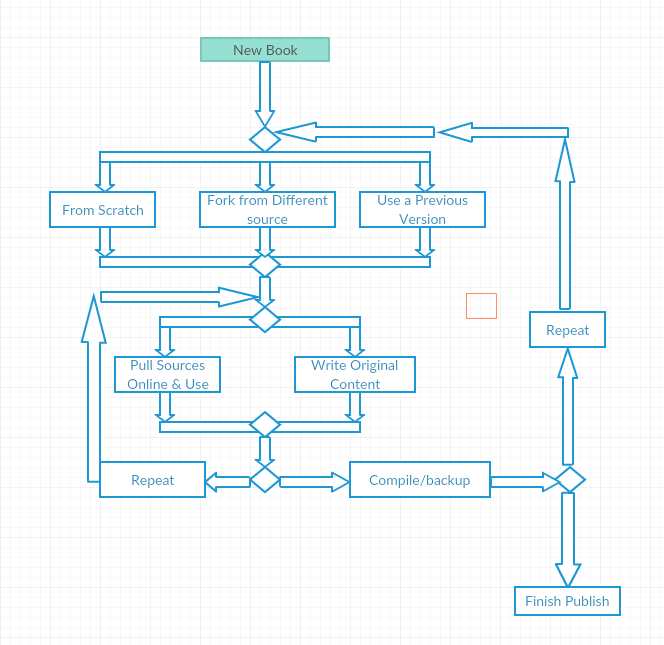
\includegraphics[width=150mm]{usage_diagram.png}
\caption{A preliminary UML Diagram that outlines the basic flow of information}
\end{figure}

\bigskip

\newpage
\bibliographystyle{IEEEtran}
\bibliography{requirements}

\newpage
\centerline{\sc \large Signature Page}
\vspace{5pc}


\centering

\begin{tabular}{lllll}
Dr. Carlos Jensen, Client    & \_\_\_\_\_\_\_\_\_\_\_\_\_\_\_\_\_\_\_\_\_\_\_\_\_\_\_\_\_\_\_\_\_\_ & Date & \_\_\_\_\_\_\_\_\_\_\_\_\_\_\_\_\_\_\_\_\_ &  \\
                         &                                                                                  &      &                                            &  \\ \\
Steven Powers, Developer & \_\_\_\_\_\_\_\_\_\_\_\_\_\_\_\_\_\_\_\_\_\_\_\_\_\_\_\_\_\_\_\_\_\_ & Date & \_\_\_\_\_\_\_\_\_\_\_\_\_\_\_\_\_\_\_\_\_ &  \\ 
                         &                                                                                  &      &                                            &  \\ \\
Josh Matteson, Developer & \_\_\_\_\_\_\_\_\_\_\_\_\_\_\_\_\_\_\_\_\_\_\_\_\_\_\_\_\_\_\_\_\_\_ & Date & \_\_\_\_\_\_\_\_\_\_\_\_\_\_\_\_\_\_\_\_\_ &  \\ 
                         &                                                                                  &      &                                            &  \\ \\
Evan Tschuy, Developer   & \_\_\_\_\_\_\_\_\_\_\_\_\_\_\_\_\_\_\_\_\_\_\_\_\_\_\_\_\_\_\_\_\_\_ & Date & \_\_\_\_\_\_\_\_\_\_\_\_\_\_\_\_\_\_\_\_\_ &  \\ 
                         &                                                                                  &      &                                            & 
\end{tabular}

\end{document}
